\documentclass[a4paper, 11pt]{article}
% ----- Loading the Package MCMthesis -----
% -----           v 5.01-L            -----
% `tcn' is short for `Team Control Number'.
% You should fill your tcn after the equal sign following tcn.
% The option `sheet' contorls weather the summary sheet
% will appear.
% The option `abstract' controls weather the abstract 
% will appear in the title-page.
\usepackage[tcn = 39465, sheet = true, abstract = false]{MCMthesis}
\problem{A}
\usepackage{palatino}
\setlength\parskip{.5\baselineskip}
\providecommand{\abstractname}{\relax}
\renewcommand{\abstractname}{Abstract} 

\title{MCM essay}
\author{}
\date{\today}

\begin{document}
\begin{abstract}
	The first recorded Ebola outbreak occurred in Nzara, South Sudan in 1967 which infected 284 and killed 151. Since then, Ebola outbreak occurs frequently and there are nearly 20 cases of major or massive outbreaks till now, the most recent of which is the case in Liberia, Guinea and Sierra Leone in 2014. The case fatality rate ranges from 25\%(Uganda, 2007) to 90\%(Republic of Congo, 2002). Considering its high fatality rate and damage to human society, it is highly valuable to study the property of the spread of Ebola and to find out feasible strategy to fight against the virus.

	In this paper, we attempted to untangle the convolution of parameters and variables concerning the spread of Ebola and to give a constructive suggestions regarding what strategy should be taken to deliver limited amount of drug and vaccine. Also, we planned to give an optimized plan to deliver vaccine and drug under a simplified case based on the real case of the recent outbreak in west Africa.

	We constructed models based on the biological features of EVD, social features of human society and several reasonable assumptions. Our models consist of two parts: one is considering the the spread of disease within a single city with SIR model and serves as the base of the other; the other takes the people flow among the cities into account, the application of which gave us an optimized plan regarding how should we allocate the resources of medication such as vaccine. In fact, our model is a combination of classic SIR model and graph theory, which is a simple method to solve geography related disease spread problem.

	Both of the models were applied to specific cases separately, and the results of computation which were carefully studied justified our model. Through our analysis of the model, we explored and explained the complex relationship among numerous variables and parameters. Then we find the existence of threshold values for those relationship, which indicates a limit condition for outbreak. According to the analysis and literature's instruction, we put forward our own criterion.

	The effectiveness of medical treatment (including segregation, vaccination and pharmacotherapy) is verified by our model and the strategy to allocate vaccine and drug is revealed by our investigation. Specifically, the amount of vaccine or drug delivered to each city should be roughly proportional the scale of the city and the amount of vaccine or drug allocated per capita should be larger for the cities in the center of people flow network.
\end{abstract}
\maketitle
\tableofcontents
\newpage
\pagestyle{fancy}

%======================问题介绍==================
\section{Introduction}

\par Ebola virus disease (EVD), which is also called Ebola hemorrhagic fever or simply Ebola, is an infectious disease caused by one of the Ebola virus strains, alongside high lethality and rapid epidemicity. EVD was first discovered in 1976 near the Ebola river. Since then, outbreaks have appeared sporadically in Africa. In 2014, the largest outbreak of the disease occurred in West Africa and caused thousands of cases of death.\cite{CDC} Due to the severity of its outbreak, a feasible method is required to outline its progression and to predict trends, thus being able to form a strategy fighting against infectious diseases like EVD.
\subsection{The problems we concern}
As is known to all, the spread of EVD is influenced by various factors. Knowing these factors and the role they played can give us a depper understanding of EVD. Therefore, we are eager to figure out factors influencing the spread.

Another problem lies in the delivery system of drug and vaccine. Since \emph{the World Medical Association} has announced a new medication (as is stated in the problem), the quantity and location of medication delivery became a problem of great concern. Considering that pharmaceutical industries may not capable of manufacturing enough drug and vaccine, we need to optimize the delivery plan to suppress the spread of EVD.

\subsection{The models we are to construct}
In this paper, our purpose is to construct mathematical models that can effectively solve these problems. To meet the goal, we attempt to divide the model into two main parts.

Firstly, we want to construct an initial model discussing the spread of disease in a single city. Some main factors that influence the spread of disease are considered in this model, but the influence and interaction with other cities are not included. This model can describe, at least roughly, the development of EVD in the city after some citizens are infected and measure the importance of different factors, but the spread among cities still cannot be seen. Accordingly, the optimized delivery plan cannot be made with the aim of this single model.

Secondly, we are going to construct a multiple-city model based on the first model. In this model, cities are connected by specific relation, thus allowing pathogen spreads from one city to another. This model can be used to describe the spread of disease in a rather vast geographic regions. With the aim of this model, we use genetic algorithm (GA) to optimize delivery plan.

\section{Background}
In this part, we would introduce some natural characters of EVD and historical records of EVD outbreaks. This will help us understand how it spreads and determine appropriate values for the parameters in our models, such as infection rate, recovery rate, etc.

\subsection{Characters of Ebola and its spread}

\par Many factors related to Ebola influence the spread of EVD or influence the construction of our models. These factors are divided into \textbf{Social factors} and \textbf{Biological factors} and they are listed as follows.

\subsubsection{Biological factors}
\begin{itemize}
  \item \textbf{Infectiousness }\\ Infectiousness directly affects the disease's infection rate, which is defined as morbidity rate for uninfected people but exposed to virus carriers. And infectiousness is mainly affected by virulence of the virus and individual's immunity. In most cases, diseases' infection rate is regarded as constant.\\ 
      
  \item \textbf{Lethality }\\ Lethality is how capable a disease is of causing death. It can be described by lethality rate, the ratio of the dead to the total patients. EVD has an average fatality rate of $55\%-80\%$. Moreover, Individuals who was infected and cured won't be infected again in next ten years.
       
  \item \textbf{Incubation}\\ Incubation means that there is a period during which the infected shows no sign or symptom of the disease and is not contagious\cite{CDC}. Therefore, there may be difficulty to segregate people with infectious diseases. EVD's incubation period is $2$ to $21$ days.
      
  \item \textbf{Route of Transmission} \\EVD is mainly spread through direct contact with blood and body fluids of infected ones\cite{CDC}. These routes of transmission are highly connected to public health situation and personal hygiene.
      
  \item \textbf{Environmental Condition}\\ Ebola virus has moderate tolerance to heat, which indicates that EVD maintains a high infectiousness in most of human settlements. However, Ebola virus will be inactivated when exposed to a temperature over $60^{\circ}$  for $60$ minutes. Environment also affects the spread of EVD in aspect of natural reservoir. Though the reservoir remains unknown, it is reasonable to infer that contact with wide animals adds to the probability of getting infected.
      
%  \item 

\end{itemize}


\subsubsection{Social factors}
\begin{itemize}
  \item \textbf{Population}\\In general, a large population means high potential of disease's spread. People in a populous area have a greater frequency of contacting the others than those in a sparsely populated area. According to the route of transmission, it is obvious that the probability of getting infected would be larger.
   
  \item \textbf{Traffic}\\Convinient traffic encourages population mobility, which contributes to the spread of EVD. However, It also encourages freightage, including medicine.
  
  \item \textbf{Medical Level}\\A society will be less affected by EVD if proper measures are taken efficiently and promptly.
   These measures include segregating patients and strengthening the sanitary control of public places. The manufacture of drugs and vaccines aiming at EVD is also an important part.
  
  \item \textbf{Regional Custom}\\Funeral is considered solemn in the African culture. The dead should be cleaned, kissed and touched before buried. This kind of culture facilitates EVD infections.
  
  \item \textbf{Other Social Factors}\\The spread of diseases is also influenced by factors like social development, health situation, individual's living condition, etc. These factors are not considered to simplify our models.
\end{itemize}

\subsection{Information about the last break of Ebola in 2014}

\par In 2014, the largest outbreak of the disease occurred in West Africa, affecting multiple countries mainly including Guinea, Liberia and Sierra Leone.\cite{CDC}Up to February 4th, there have been 22,495 reported confirmed, probable, or suspected cases of EVD worldwide, with 8981 reported deaths. Among these reported cases, 99.84\% of the cases (22,460) are reported in Guinea, Liberia or Sierra Leone, thus showing a strong regional characteristic and suggesting that we should focus our study mainly within these countries.
\section{Previous work}

Controlling the spread of infections is by no means a new problem, and many models have previously been used to describe the distribution and spread of epidemic diseases.

The models previous scientists used can mainly be divided into three categories. Brief overviews of the three by the sequence of their advent are as follows.
\begin{enumerate}
	\item \textbf{\emph{Standard SIR(susceptible-infected-removed) models and its deriveratives:}}The model is first put forward by \textbf{Kemraek} and \textbf{MeKendriek} in 1927\cite{SIR}and is the most classic model. Many successive models are based on it. It regards the epidemic area as a whole and divides people into different groups, such as susceptible group, infected group and removed group. It depends on differential equations to describe the relationship between volumes of different groups, thus making scientific and quantitative description. Details of the model will be explained in the successive sections.
	      \par Many other models are derived from this very basic SIR model, such as SIS model\cite{SIS} which deals with situations where a infected and later recovered individual can turn back to be a susceptible individual, and SEIR model\cite{SEIR} which deals with the situations where incubation period of the epidemic disease is not negligible. Previous scientists gained great achievements by using SIR model - they simulated the trends of epidemic diseases, calculated the rough volume of each group in different periods of epidemics and, most importantly, successfully analyse the contribution of different parameters to stability of system.
	      \par Despite the fundamental and important standing of SIR model, its drawbacks are easy to realize. It is difficult to study geographic characters of the spread of diseases, because the model doesn't contain any geographic information. Also, each person in the system is not individually recognized and the complex relationships among individuals are hardly considered, since it regards the epidemic area as a homogeneous system - in another word, each person in the system is just like a molecule in a cup of water and the relationships of any two pairs are identical. Additionally, it is a deterministic model witch hardly resemble the factual system in which many fortuitous factors matter.
	\item \textbf{\emph{Statistical model:}}This model is less intensely studied than the other two models. In this model, researchers mainly use possible functions whose forms are known but parameters unknown to fit the currently available data, aiming at predicting the trend of epidemics. Although the model is somewhat phenomenological and catch little intrinsic logic, it is quite useful in real practice and it allows us to have a quick view of the trend without getting convoluted into the depth of the problem. Anyhow, we will not go further into this kind of models.
	\item \textbf{\emph{Spatial simulation model:}}This category of models are the focus recently. They mainly contains models using cellular automaton (CA), models considering networks among people(eg. small world network), models using GIS\cite{GIS}, etc. Take models using CA as an example. We define different types of points, which are put in lattices of a plane, and regard the spread of diseases between people as the interaction between nearby points. The process of evolution and spatial distribution of virus can be simulated with the aid of computer program. Clearly, due to the consideration of individuals separately, the results are more accurate than previous two categories.

	      This category of models taking the relationship among people and geographic information into account has advantages over others when figuring out the geographic characters of the spread. Moreover, it can give more accurate results since its high resemblance of real situation. Accurate as the models are, they are highly complicated and some of them are difficult to apply both for the complexity of programming and great amount of computation.
\end{enumerate}
\section{Model for multiple cities}
In previous section we have constructed a model based on classic SIR model. This model, however, cannot give us more information about geographic spread of epidemic disease, thus contributing little to settle the problem how drugs and vaccines should be allocate. Hence, we propose a model considering geographic and demographic data in different cities. This model is on the base of previous single-city model, in another word, we suppose that in each individual city, the spread of the epidemic disease follows the single-city model previously constructed in the previous section. In addition, people flows among cities are added in to previous model.

\subsection{Symbols}
Symbols that newly appear in this section are listed in table \ref{tab.symbol2}. Some of the symbols in table \ref{tab.symbol} are also used in this section and are not listed here.
\begin{table}[htbp]
	\centering
	\begin{tabular}{|l|l|}
		\hline
		Symbol & Defination \\
		\hline
		$\mathcal{N}_i$ & total volume of population in city $i$\\

		$\mathcal{S}_i$ & number of susceptible people in city $i$\\

		$\mathcal{I}_i$ & number of infected but not segregated people in city $i$\\

		$\mathcal{G}_i$ & number of segregated and also infected people in city $i$\\

		$\mathcal{D}_i$ & number of death caused by EVD in city $i$\\

		$\mathcal{R}_i$ & number of recovered people (also immunized) in city $i$\\

		\textbf{$P_{i}$} & Total number of people in city $i$ apart from the people who are \\ & dead and segregated \\

		\textbf{$t_{i,j}$} & number of people transmit from city $i$ to city $j$ indeed \\

		\textbf{$\alpha$} & transmission coefficient \\

		\textbf{$d_{i,j}$} & distance from city $i$ to city $j$ \\

		$vacc_{tot}$ & the number of shares of vaccine that can be provided to all the cities every day\\

		$vacc_{i}$ & the number of shares of vaccine that can be provided to city $i$ every day\\
		\hline
	\end{tabular}
	\caption{The definition of the symbols.}  \label{tab.symbol2}
\end{table}

%======================假设==================
\subsection{Assumptions}
\begin{itemize}
	\item \textbf{People flow exists between any two cities }\\
	      Because no city would be quarantined totally in reality, there is connection between any two cities more or less, which means that there are flows of people between any two cities, although few people are flowing from one far-away small town to another.
	\item \textbf{Cities are different}\\
	      To analyze the influence of delivery plan of medicines, it is better to consider that the population, location and initial status of each cities are different. To make our model realistic, we analyzed the last breakout of Ebola in west Africa in 2014 and chose some cities in the epidemic area. We consider information including geographic location, population of cities and distance between cities.
	\item \textbf{Deterministic factors of people flow}\\
	      We assume that quantities of people leaving one city remains constant. Considering that the cities are laying on a 2-D plane, the intensity of people flow from one city to another is obviously inversely proportional to the distance between the two cities.

	      We also assume that, for any individual, the probability of the one go out and link with (go to another city to visit friends, handle business affairs, etc.) any other individual are equal. Hence, it comes out that the people flow from one city to another is proportional to the product of populations of the two cities.

	\item \textbf{Several properties of the system are time independent}\\
	      To simplify our model, we assume that the quantities of drugs and vaccines delivered to each city per day are determined at the beginning and would not change with time. It means that the daily received quantity of drugs and vaccines for each city are constant. %This assumption is based on the engineering control program. Once the delivery plan has been decided, it would not change everyday because of too much sources wasting on the change.

	      We assume that the birth rate and natural mortality rate are generally equilibrium and fatality due to the disease is negligible compared with total population. It comes out that the total population (including fatality) is unchanging with time and the people flow among cities is also time independent.

	\item \textbf{The segregated and dead would not transmit from one city to another}\\
	      The S(Segregated) and D(dead due to the epidemic disease) are certainly not able to go from one city to another. Hence, when we calculated how many people from specific group are transmitted from one city to another, only the other three groups (the susceptible, the infected but not segregated, and the recovered and immunized) are taken into account.
\end{itemize}

\subsection{Construction of general model considering multiple cities}
This model considering multiple cities are based on the previous single-city model. The difference between them is that in this multi-city model we consider the people flow among cities.

Under assumptions previously mentioned, it is easy to conclude that the number of people transmitted from one city to another can be determined by
\begin{equation}
	t_{j,i} = t_{i,j}=\alpha \cdot\frac{1}{d_{i,j}}\cdot P_{i}\cdot P_{j}
\end{equation}
where
\begin{equation}
	P_{i}=\mathcal{S}_{i}+\mathcal{I}_{i}+\mathcal{R}_{i}
\end{equation}
$\alpha$ is transmission coefficient which is a constant among all the cities, and $t_{i,j}$ is the number of people transmitted from city $i$ to city $j$.

Different groups of people that are transmitted among cities are proportional to their proportion in departure city. Explicitly, for each day,
\begin{align}\label{group}
	\mathcal{S}_{j} & =\mathcal{S}_{j}+\sum_i \frac{\mathcal{S}_{i}}{P_{i}}\cdot t_{i,j} \\
	\mathcal{I}{j}  & =\mathcal{I}_{j}+\sum_i \frac{\mathcal{I}_{i}}{P_{i}}\cdot t_{i,j} \\
	\mathcal{R}_{j} & =\mathcal{R}_{j}+\sum_i \frac{\mathcal{R}_{i}}{P_{i}}\cdot t_{i,j}
\end{align}

Hence, previous derived difference equations can be written as
\begin{subequations}
	\begin{align}
		\dfrac{\mathcal{S}_{i+1} - \mathcal{S}_{i}}{\Delta t} & =-\frac{h}{\sigma}\mathcal{S}_i\mathcal{I}_i-\frac{vacc}{\sigma}+\sum_i \frac{\mathcal{S}_{i}}{P_{i}}\cdot t_{i,j}                    \\
		\dfrac{\mathcal{I}_{i+1} - \mathcal{I}_{i}}{\Delta t} & =\frac{h}{\sigma}\mathcal{S}_i\mathcal{I}_i-\frac{(k_1+g+r_s)}{\sigma}\mathcal{I}_i+\sum_i \frac{\mathcal{I}_{i}}{P_{i}}\cdot t_{i,j} \\
		\dfrac{\mathcal{G}_{i+1} - \mathcal{G}_{i}}{\Delta t} & =\frac{g}{\sigma}\mathcal{I}_i-\frac{k_2}{\sigma} \mathcal{G}-\frac{r_g}{\sigma} \mathcal{G}                                          \\
		\dfrac{\mathcal{R}_{i+1} - \mathcal{R}_{i}}{\Delta t} & =\frac{r_s}{\sigma}\mathcal{I}_i+\frac{r_d}{\sigma} \mathcal{G}_i+\sum_i \frac{\mathcal{R}_{i}}{P_{i}}\cdot t_{i,j}                   \\
		\dfrac{\mathcal{D}_{i+1} - \mathcal{D}_{i}}{\Delta t} & =\frac{k1}{\sigma}\mathcal{I}_i+\frac{k_2}{\sigma} \mathcal{G}_i
	\end{align}
\end{subequations}

\subsection{Numerical Computation of general model considering multiple cities}
At first, we exam the multi-city model with a simplified situation in which the quantities of drugs and vaccines delivered to each city are the same. We will show that it properly figures out the general trend of the spread of disease among cities and show us some significant character of the process.
\subsubsection{Process of numerical computation}
The steps of calculation are listed below:
\begin{enumerate}
	\item \textbf{Initial conditions}
	\item \textbf{Calculation based on single-city model for each city }
	\item \textbf{Simulate people flows among cities}
	\item \textbf{Repeat Step 2 and Step 3 for the next moment}
	\item \textbf{Until the preset $days$}
\end{enumerate}
In fact, from single-city model to multiple-city model, we simply added step 3.

Other parameters that we are used in the computation, if not stated specifically, are the same as single-city model. For clarity, we also list them here.

$\beta = 0.32$ , $k_1 = 0.023$, $r_s = 0.0103$ , $days = 150$ ,  $\Delta t = 0.1 (\text{days})$.

\subsubsection{Selection of geographic data}
Since the outbreak of EVD are usually constrained in regional areas (mentioned in background), the geographic data that we selected to simulate the last break of EVD is all from the three countries in west Africa (Guinea, Liberia and Sierra Leone). There are 145 cities in these three countries (geographic locations are plotted in figure \ref{allcity}). If all taken into account, it is not only beyond the computational ability of our computers, but also, even if results are given, is difficult for us to study the details of the results. Hence, we select 18 representative cities, among which there are big cities and also small towns; there are cities that are close to each other and there are cities far away. The data of the selected 18 cities are listed in table \ref{citylist}. For the convince of later analysis, a visualized version of data of the cities are ploted in figure \ref{cityplot}.

\begin{figure}
	\centering
	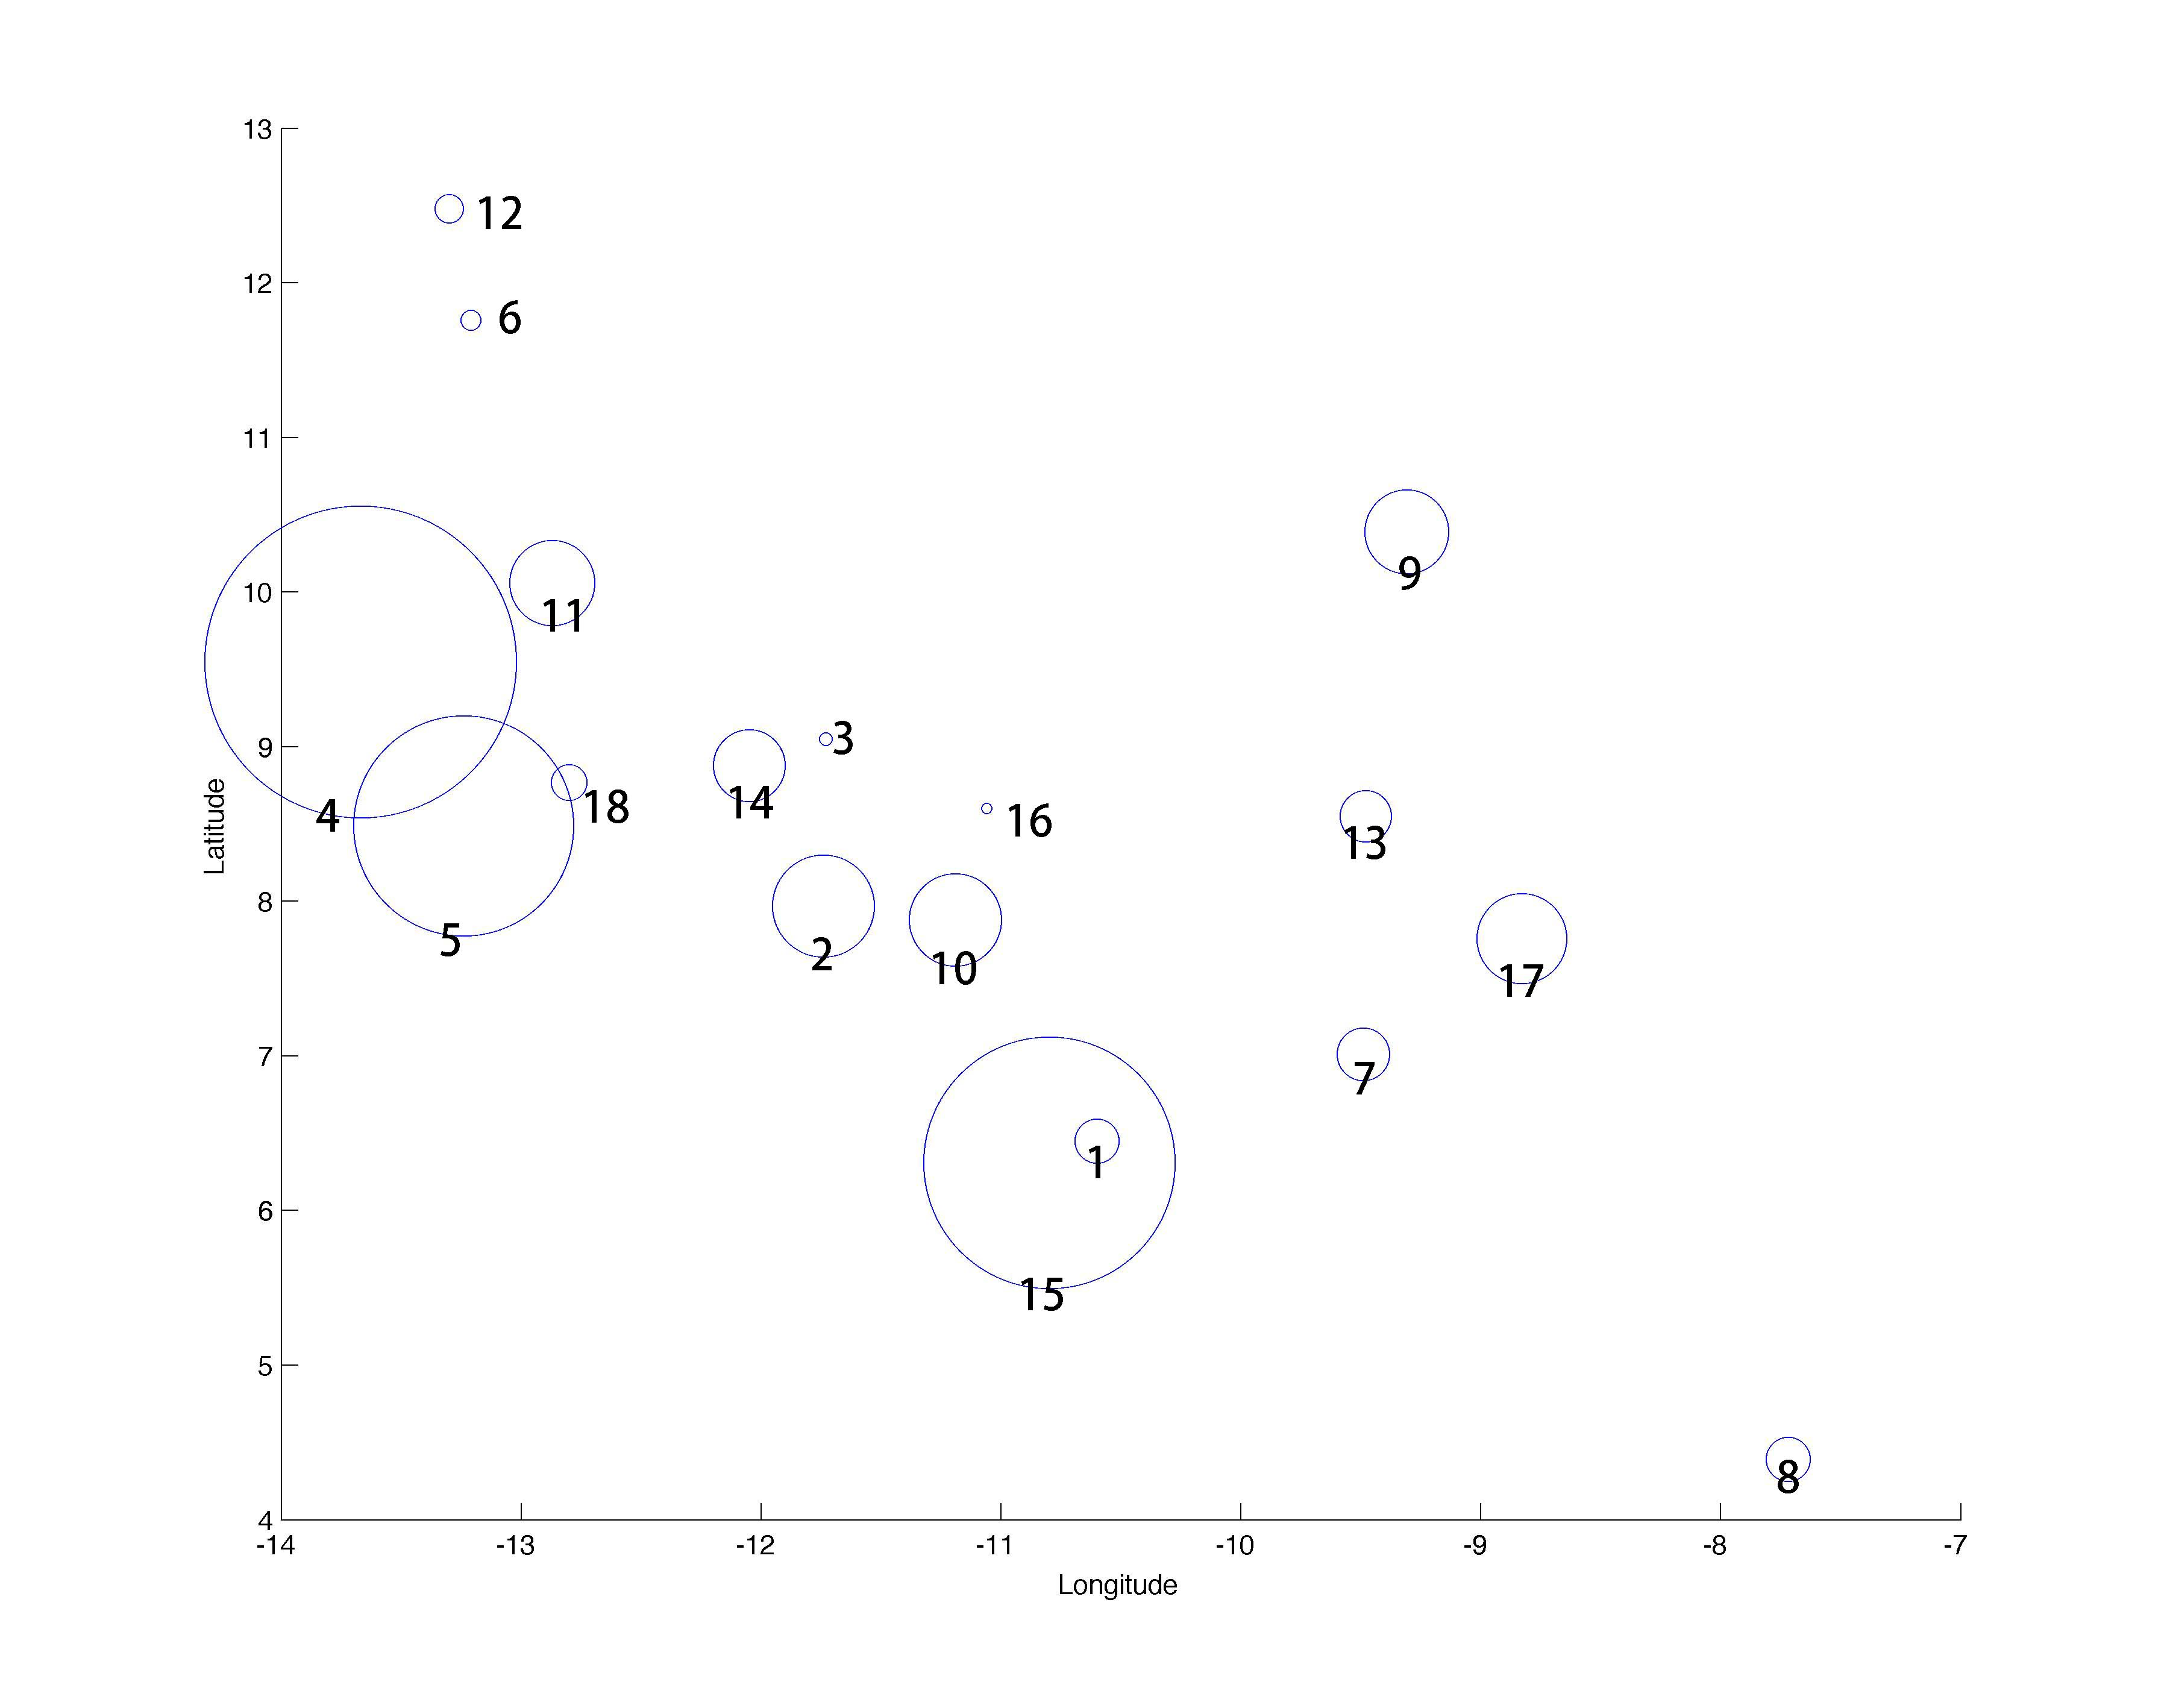
\includegraphics[width = 0.8\textwidth]{CityPopulationlabel.jpg}
	\caption{Information of 18 selected cities. Each circle stands for a city - the center of circle stands for location and the area of circle stands for population. The labels on or nearby the circles are corresponding to the labels in table \ref{citylist}}
	\label{cityplot}
\end{figure}

\begin{figure}
	\centering
	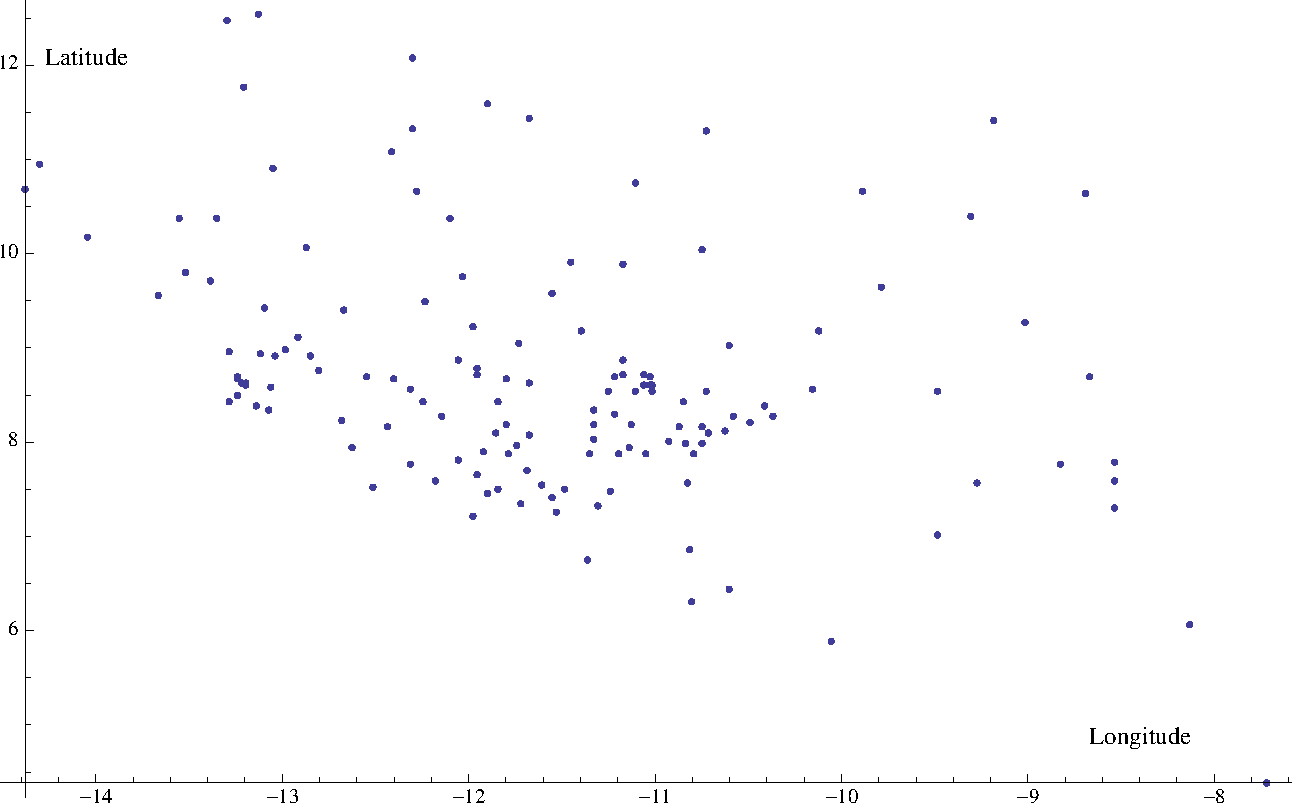
\includegraphics[width = 0.6\textwidth]{allcity.pdf}
	\caption{Locations of cities in the three countries}
	\label{allcity}
\end{figure}

\begin{table}[htb]
	\centering
	\begin{tabular}{|r|r|r|r|r|r|r|}
		\hline
		Label & City               & Province/Region    & Country            & Latitude & Longitude & Population \\
		\hline
		1     & \text{Bensonville} & \text{Montserrado} & \text{Liberia}     & 6.45     & -10.6     & 33188      \\
		2     & \text{Bo}          & \text{Southern}    & \text{SierraLeone} & 7.97     & -11.74    & 167144     \\
		3     & \text{Bumbuna}     & \text{Northern}    & \text{SierraLeone} & 9.05     & -11.73    & 3222       \\
		4     & \text{Conakry}     & \text{Conakry}     & \text{Guinea}      & 9.55     & -13.67    & 1548470    \\
		5     & \text{Freetown}    & \text{Western}     & \text{SierraLeone} & 8.49     & -13.24    & 772873     \\
		6     & \text{Gaoual}      & \text{Gaoual}      & \text{Guinea}      & 11.76    & -13.21    & 7461       \\
		7     & \text{Gbarnga}     & \text{Bong}        & \text{Liberia}     & 7.01     & -9.49     & 45835      \\
		8     & \text{Harper}      & \text{Maryland}    & \text{Liberia}     & 4.39     & -7.72     & 32661      \\
		9     & \text{Kankan}      & \text{Kankan}      & \text{Guinea}      & 10.39    & -9.31     & 114009     \\
		10    & \text{Kenema}      & \text{Eastern}     & \text{SierraLeone} & 7.88     & -11.19    & 137696     \\
		11    & \text{Kindia}      & \text{Kindia}      & \text{Guinea}      & 10.06    & -12.87    & 117062     \\
		12    & \text{Koundara}    & \text{Koundara}    & \text{Guinea}      & 12.48    & -13.3     & 13990      \\
		13    & \text{Macenta}     & \text{Macenta}     & \text{Guinea}      & 8.55     & -9.48     & 43102      \\
		14    & \text{Makeni}      & \text{Northern}    & \text{SierraLeone} & 8.88     & -12.05    & 85017      \\
		15    & \text{Monrovia}    & \text{Montserrado} & \text{Liberia}     & 6.31     & -10.8     & 1010970    \\
		16    & \text{Ndoyogbo}    & \text{Eastern}     & \text{SierraLeone} & 8.6      & -11.06    & 1870       \\
		17    & \text{Nzerekore}   & \text{Nzerekore}   & \text{Guinea}      & 7.76     & -8.83     & 132728     \\
		18    & \text{PortLoko}    & \text{Northern}    & \text{SierraLeone} & 8.77     & -12.8     & 21961      \\
		\hline
	\end{tabular}
	\caption{Information of the 18 selected cities}
	\label{citylist}
\end{table}

\subsubsection{Results of numerical computation}
Similarly, we observed both outbreak situations and well-controlled conditions when we change any one of the four independent variables($g$, $drug$, $vacc$ and $C$).

Figure \ref{multibreak} shows clearly how the outbreak of disease spread from one city to another. We have observed that: 1) the order of severity (measured by fatality) is larger in the city which is the onset of disease (in our special case it is city 1) ; 2) epidemic outbreak occurs earlier in the city which is the onset of disease, in another word, the general trend of others has somewhat 'lag effect'; 3) the general trend of the city close to the onset of disease resembles more to the onset of disease in terms of severity and time sequence (in our special case it is city 15).

\begin{figure}
	\centering
	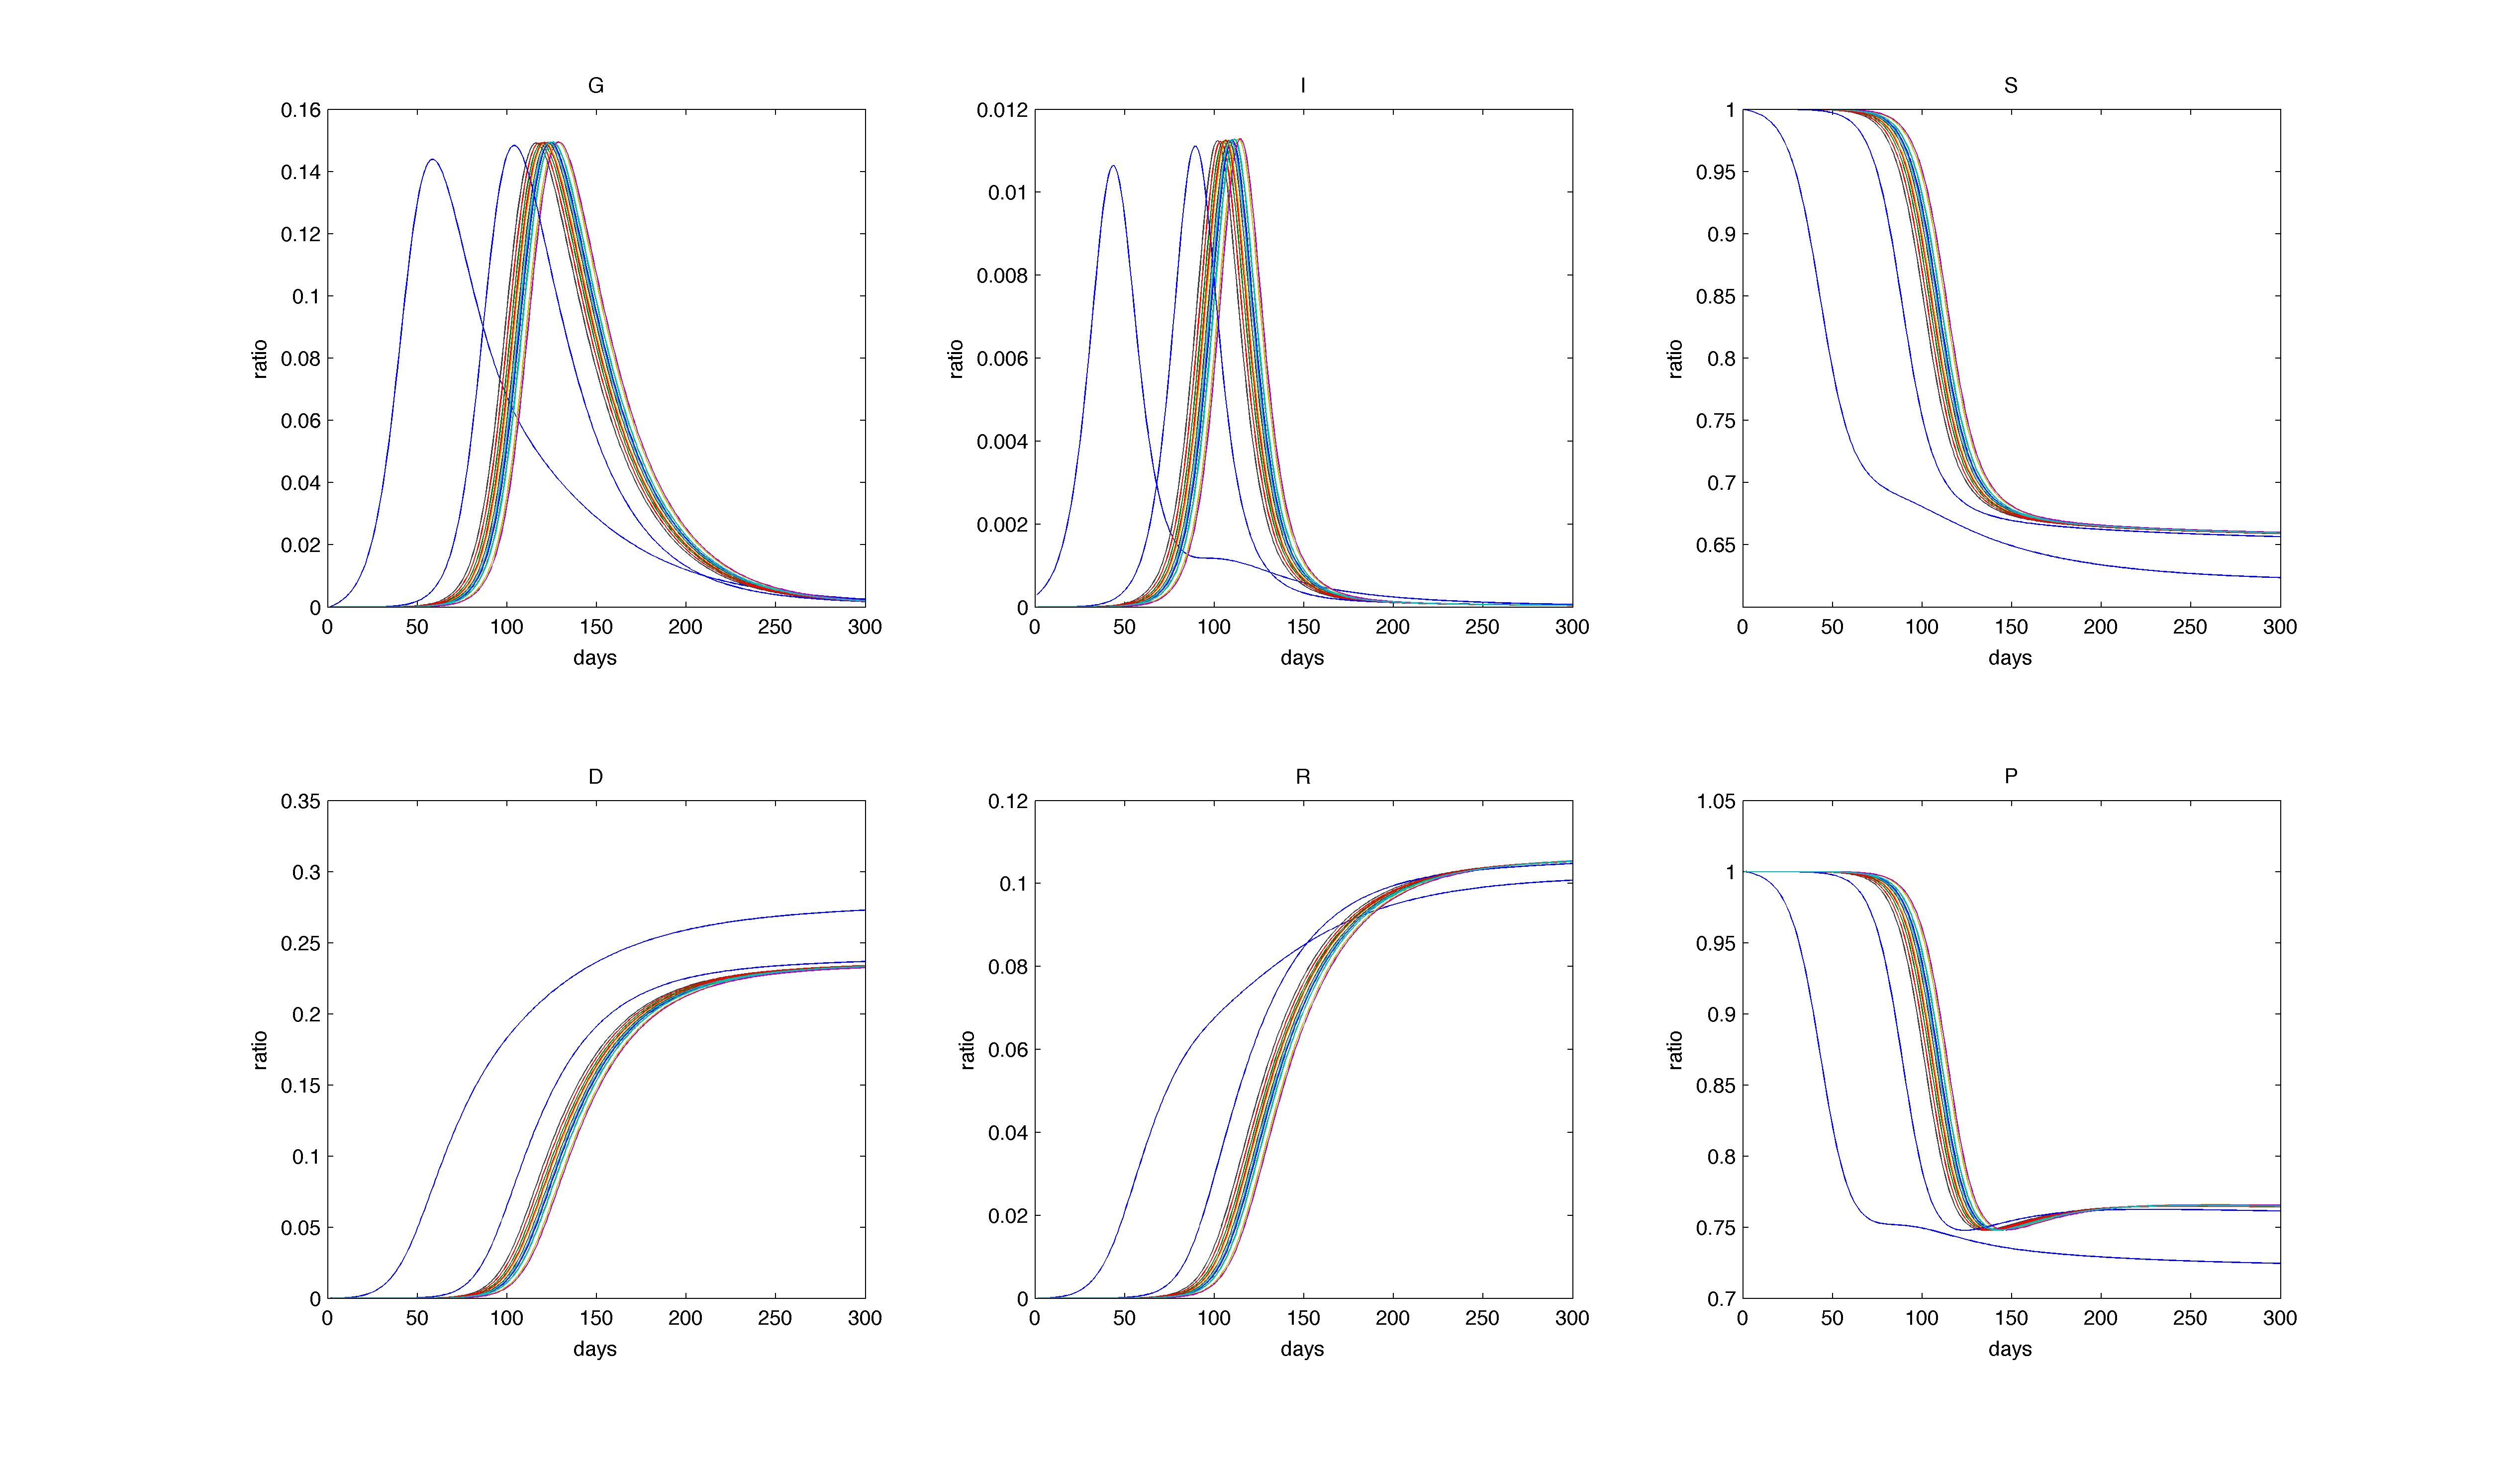
\includegraphics[width = 0.8\textwidth]{multibreak.jpg}
	\caption{epidemic disease breakout in different cities. $days = 300$, $\alpha = 10^{-4}$ , $drug = 0, vacc = 0, C = 3, g = 0.8$ and the y axis is the number of people in the group divided by the total number of people in corresponding city. Initially, 10 people are infected in city 1, and all the other people in all the cities are susceptible. The dark blue line far away from others represents city 1. The next dark blue line which is easy to distinguish from others represents city 15 which is geographically close to city 1.}
	\label{multibreak}
\end{figure}

Figure \ref{multicontrol_1000vacc} shows that when giving vaccines to the cities, the severity greatly decreases, which indicates the great influence medication has on the spread of disease. Additionally, we have observed a new phenomenon that big cities are more easy to get influenced by epidemic diseases if all the cities are given identical amount of drug or vaccine. In our special case, the trend of city 4 is showing the phenomenon. Similar features are observed when varying the value of $drug$, $C$, or $g$.

\begin{figure}
	\centering
	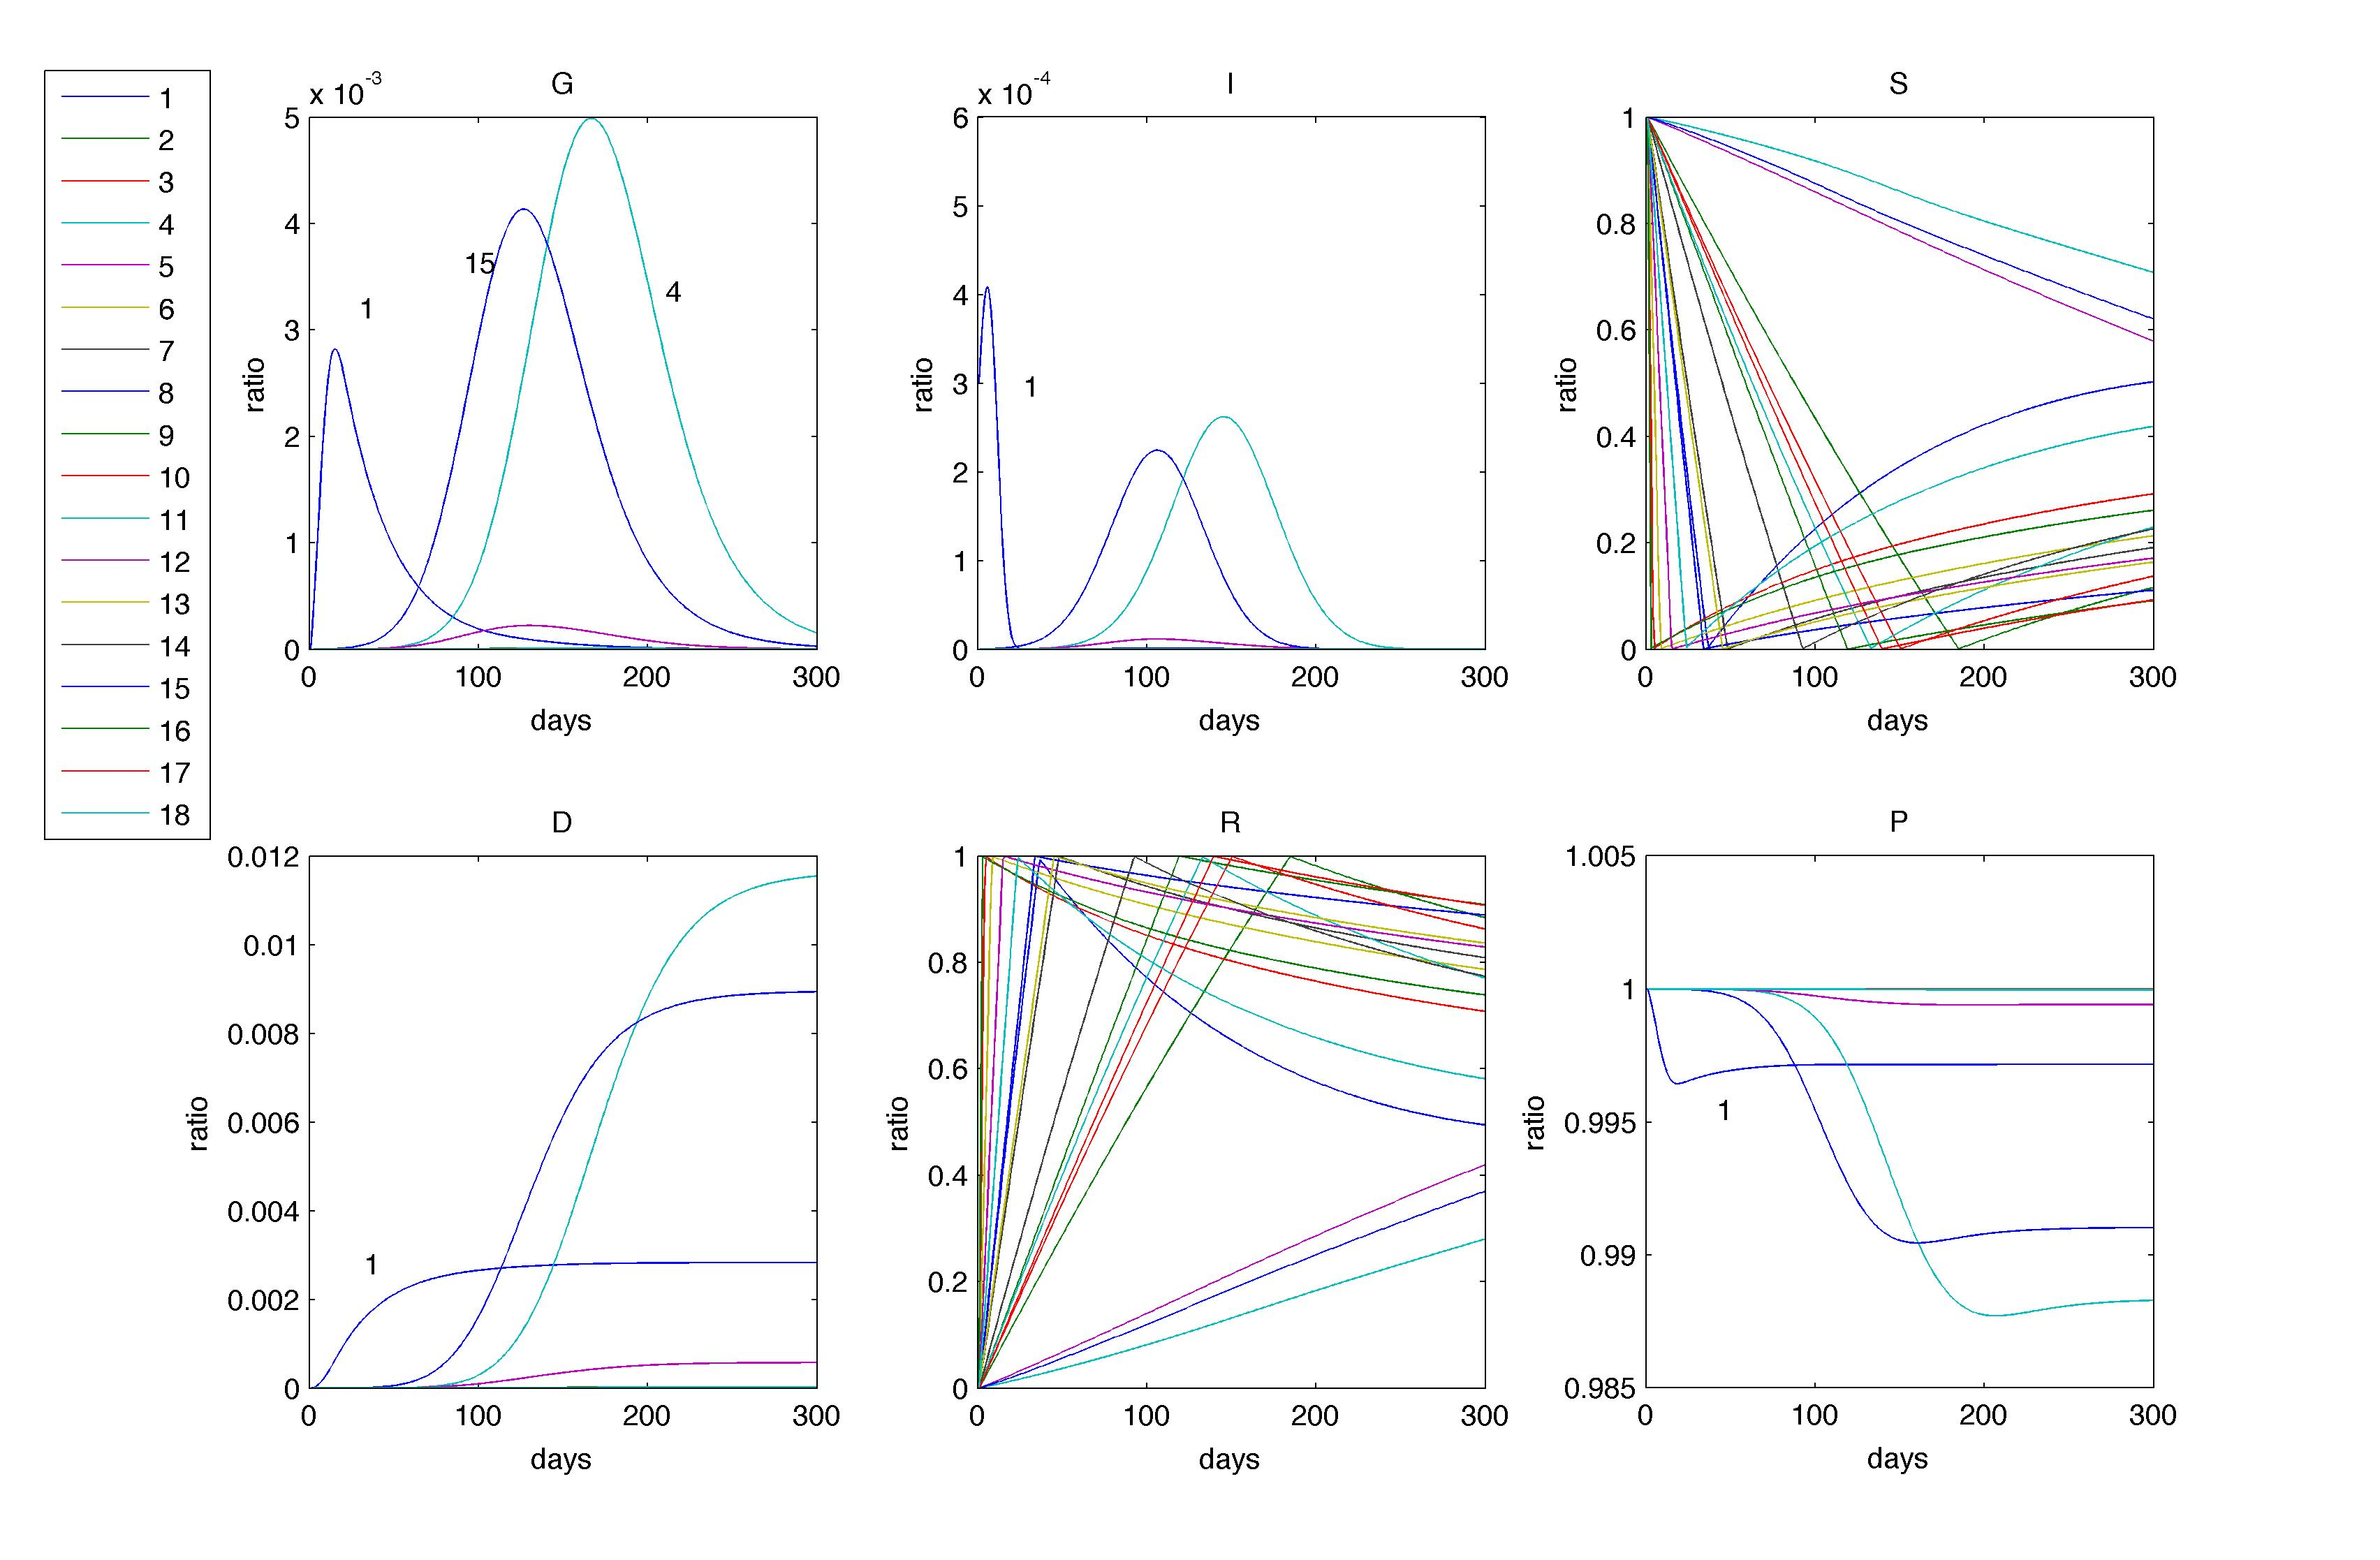
\includegraphics[width = 0.8\textwidth]{multicontrol_1000vacc.jpg}
	\caption{epidemic disease breakout in different cities. $days = 300$, $\alpha = 10^{-4}$ , $drug = 0, vacc = 1000, C = 3, g = 0.8$ and the y axis is the number of people in the group divided by the total number of people in corresponding city. Initially, 10 people are infected in city 1, and all the other people in all the cities are susceptible. The dark blue with label '1' represent city 1. The other dark blue line represents city 15 which is geographically close to city 1. The light green line with label '4' represent city 4 which is the biggest city in the all 18 cities.}
	\label{multicontrol_1000vacc}
\end{figure}

The observed phenomenon also indicates that some of the cities need more medications than the others. Hence, a carefully organized plan to delivery drugs and vaccines is needed, which will be discussed next.

\subsection{Model for optimizing the medication plan}
We have seen that different medication plans (the plans to allocate drugs and vaccines) can influence the severity of the spread of disease (measured by the total death due to the disease). Hence, here comes the question: how can we develop a plan that can reduce the number of death as much as possible.

Let us first consider a practical problem where the amount of vaccine that can be provided every day is a constant $vacc_{tot}$ (in the later computation we set the value to $vacc_{tot} = 1800$), and we are required to find out a plan to allocate the vaccines in order that the total death is as small as possible.
\subsubsection{Genetic algorithm}
Since there are many degrees of freedom of the possible plans, it is justifiable for us to use optimization algorithm to solve the problem. In order to use genetic algorithm, which is one of the most effective optimization algorithm, it is required that the degree of freedom of the plan which is to be optimized should be encoded into the form of binary `chromosome`. We encoded them into a 180-bit chromosome which is illustrated in figure \ref{chromosome}. The 180-bit chromosome is divided into 18 segments, each of which is representing the amount of vaccines that can be allocated to a city. The length of each segment representing a single city is $chromoUnitLength=10$, which is capable of donating value from 0 to $2^{10}-1$. We may as well donate the value of city $i$ as $w_i$, Hence, we can decide the amount of vaccines each city can get. The number of shares of vaccines that city $i$ can get per day is
\begin{equation}
	vacc_i = \dfrac{w_i}{\sum_{j=1}^{18} w_j} vacc_{tot}
\end{equation}

\begin{figure}
	\centering
	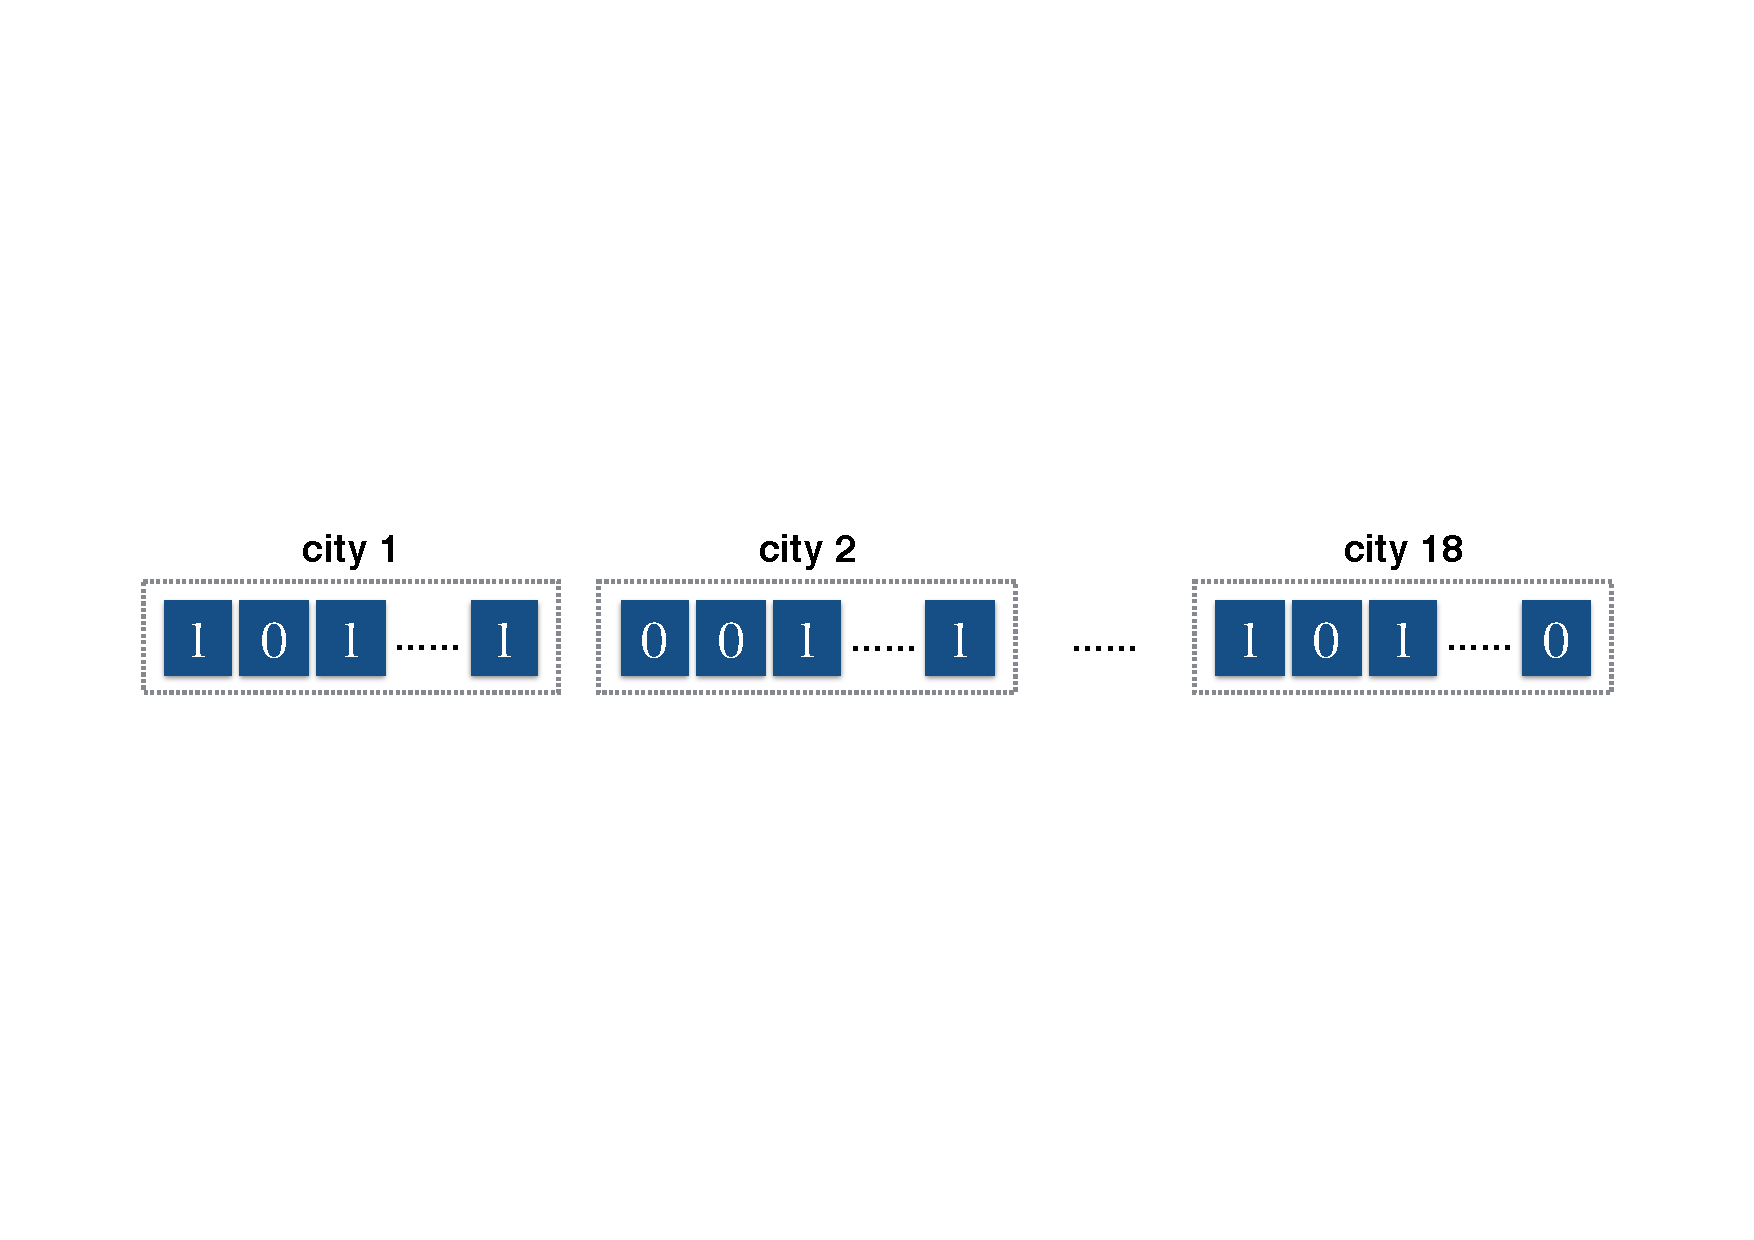
\includegraphics[width = \textwidth]{chromosome.pdf}
	\caption{Encoding}
	\label{chromosome}
\end{figure}

The process of genetic algorithm we adopted are shown in figure \ref{GA}.

On the stage of initialization (step 1 labeled in the figure), we set the number of generations to be calculated to $generationNum = 1000$, the number of individuals in each generation to $popSize = 200$, the rate of mutation to $mutationRate = 0.01$ and the rate of crossover to $crossoverRate = 0.6$.

On the stage of calculating fitness (step 2), we set the fatality rate as the target function and take it as the value of fitness.

The stage of selecting, crossover and mutation (step 3,4 and 5) are conform the very classic process of genetic algorithm.

\begin{figure}
	\centering
	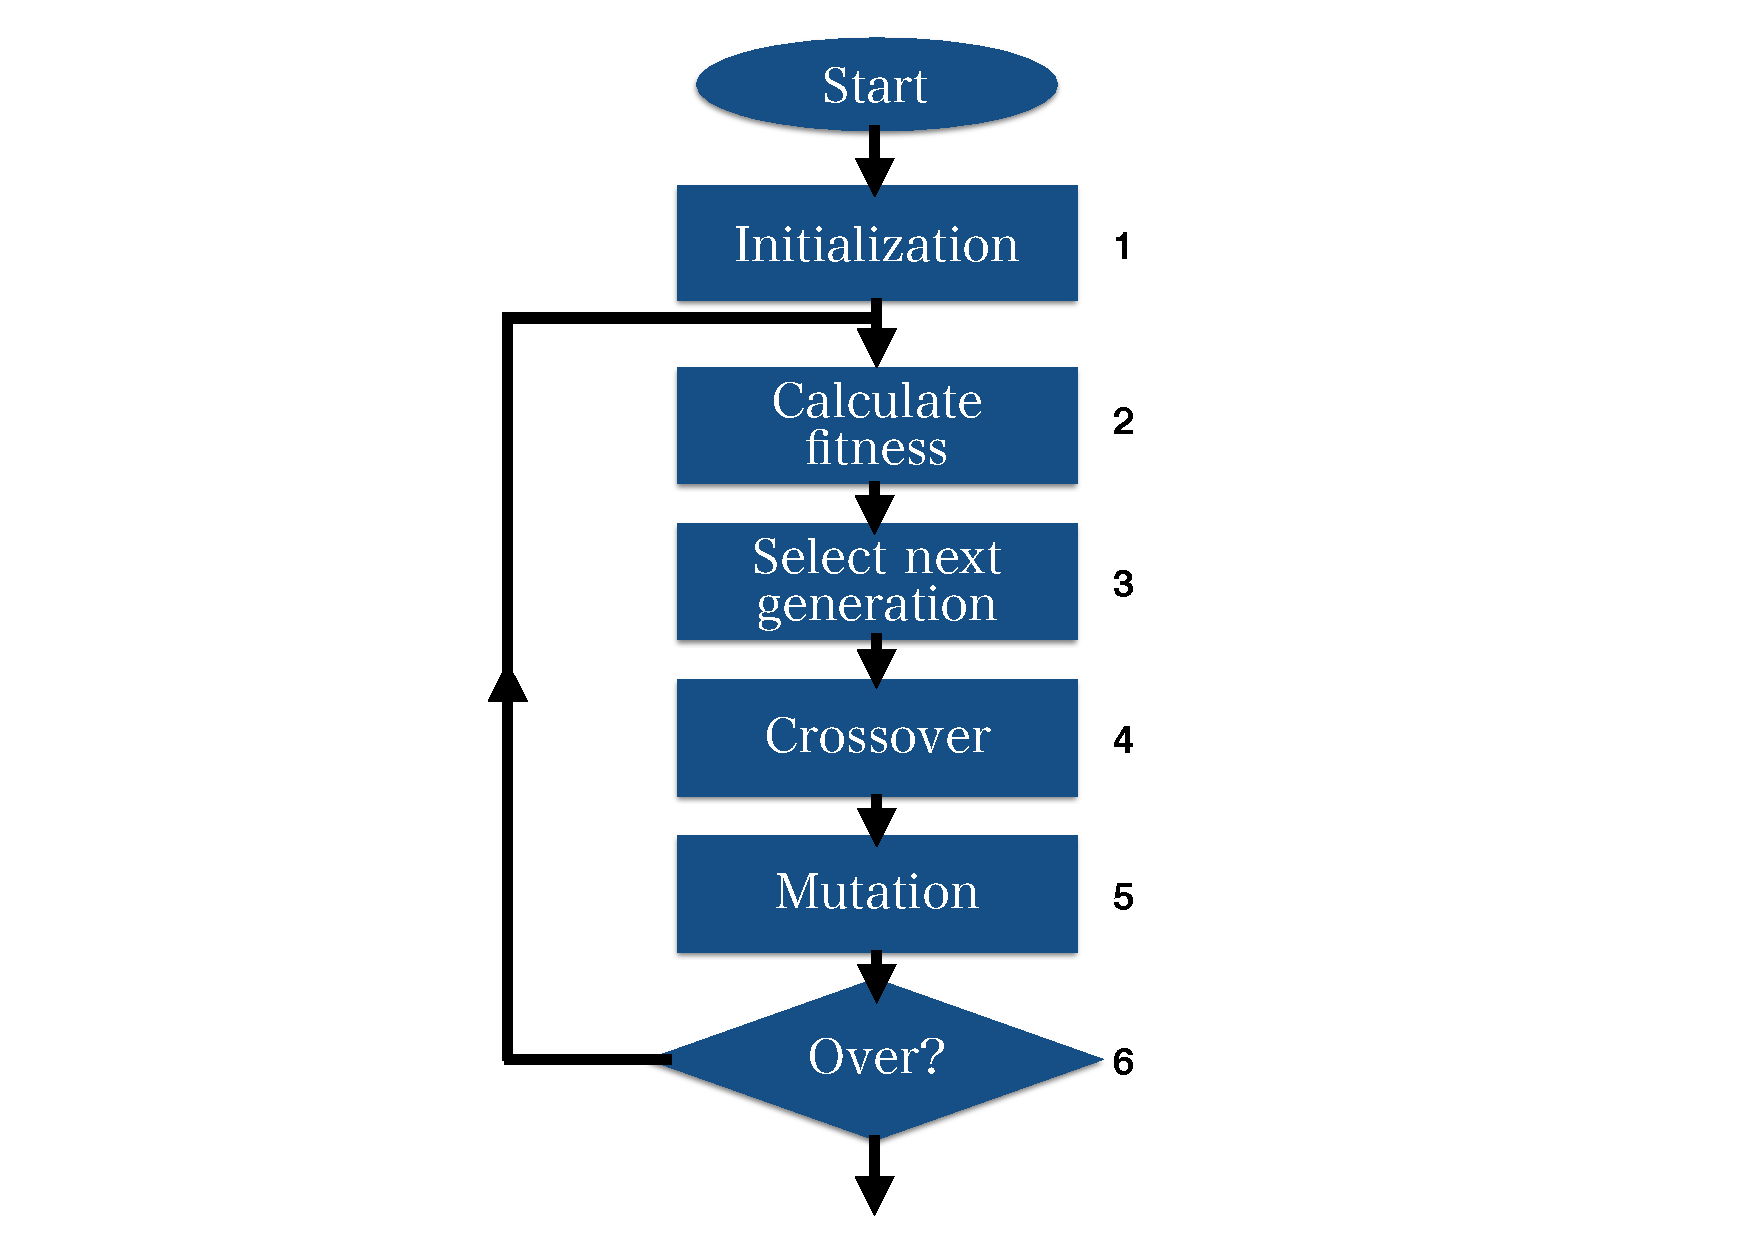
\includegraphics[width = 0.6\textwidth]{GA.pdf}
	\caption{The process of genetic algorithm}
	\label{GA}
\end{figure}

\subsubsection{Results of computation}
With parameters shown in table \ref{comppara}. A optimized result is given by our program, which is shown in table \ref{result}.

The number of death declined from 2768 with randomly generated plan to 380 with the optimized plan shown in table \ref{result}. The declining trend can be easily seen in figure \ref{fitness_avg}.

\begin{table}[]
	\centering
	\begin{tabular}{ccccccccc}
		\hline
		$\beta$ & $k_1$ & $r_s$  & $days$ & $\Delta t$ & $g$ & $C$ & $drug$ & number of initial infected people \\
		0.32    & 0.023 & 0.0103 & 150    & 0.1        & 0.8 & 3   & 0      & 10(in city 1)                     \\
		\hline
	\end{tabular}
	\begin{tabular}{cccccc}
		\hline
		$vacc_{tot}$ & $chromoUnitLegth$ & $generationNum$ & $popSize$ & $mutationRate$ & $crossoverRate$ \\
		1800         & 10                & 1000            & 200       & 0.01           & 0.6             \\
		\hline
	\end{tabular}
	\caption{Parameters in computation}
	\label{comppara}
\end{table}

\begin{table}[]
	\centering
	\begin{tabular}{|r|r|r|r|}
		\hline
		label of city & $vacc_i$ & population of city & vaccine per capita ($\times 10^{-3}$) \\ \hline
		1             & 32       & 33190              & 0.96983                               \\ \hline
		2             & 367      & 167100             & 2.1956                                \\ \hline
		3             & 3        & 3222               & 0.9082                                \\ \hline
		4             & 315      & 1548000            & 0.20345                               \\ \hline
		5             & 185      & 772900             & 0.23947                               \\ \hline
		6             & 55       & 7461               & 7.4029                                \\ \hline
		7             & 40       & 45840              & 0.86178                               \\ \hline
		8             & 14       & 32660              & 0.41439                               \\ \hline
		9             & 31       & 114000             & 0.26952                               \\ \hline
		10            & 98       & 137700             & 0.71456                               \\ \hline
		11            & 41       & 117100             & 0.34673                               \\ \hline
		12            & 94       & 13990              & 6.7195                                \\ \hline
		13            & 24       & 43100              & 0.55164                               \\ \hline
		14            & 48       & 85020              & 0.5679                                \\ \hline
		15            & 329      & 1011000            & 0.32562                               \\ \hline
		16            & 51       & 1870               & 27.1889                               \\ \hline
		17            & 27       & 132700             & 0.20398                               \\ \hline
		18            & 47       & 21960              & 2.132                                 \\ \hline
	\end{tabular}
	\caption{A optimized plan for allocating vaccine with $vacc_{tot} = 1800$ }
	\label{result}
\end{table}

\begin{figure}
	\centering
	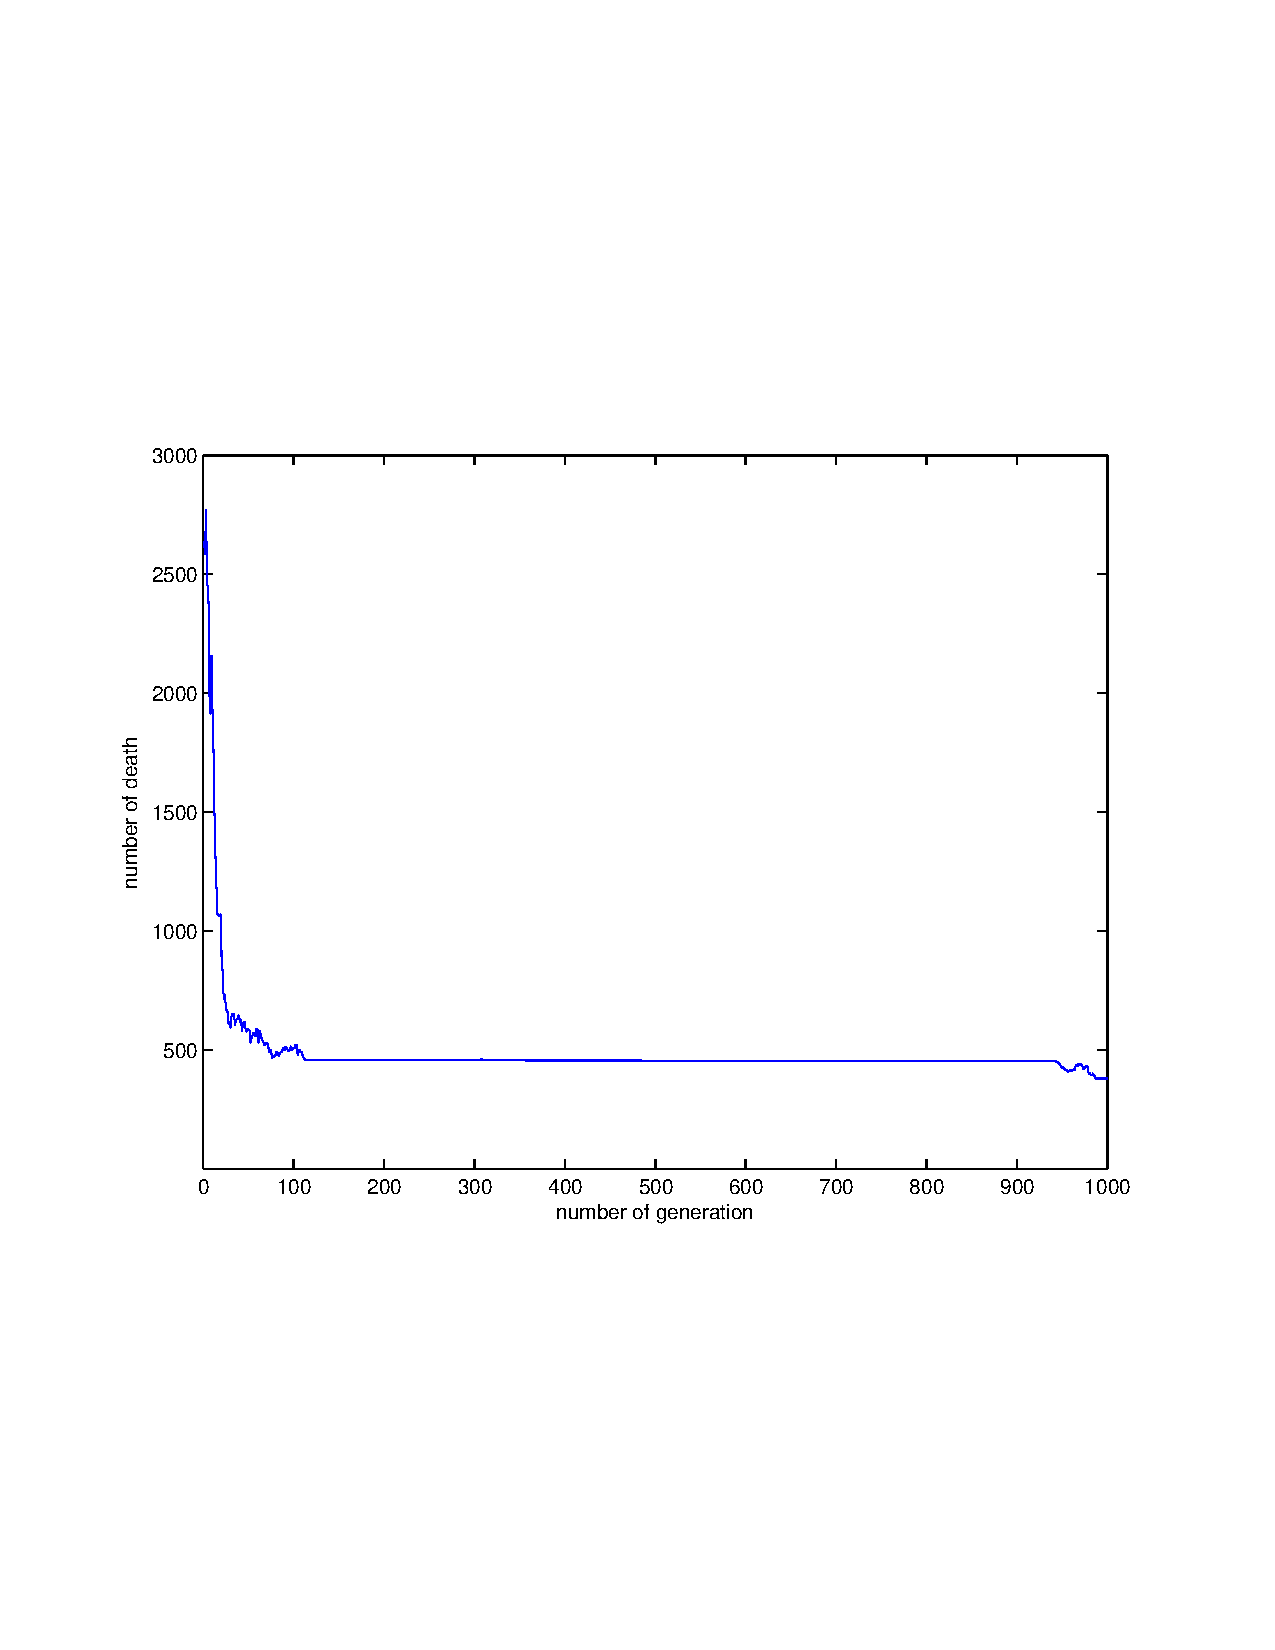
\includegraphics[width = 0.6\textwidth]{fitness_avg.pdf}
	\caption{The number of death declines with the optimization of the plan. The x axis is for the number of generations of genetic algorithm and the y axis is for the number of death in all the 18 cities.}
	\label{fitness_avg}
\end{figure}

\subsubsection{Analysis of the result}
The result is analyzed from following aspects.
\begin{enumerate}
	\item The two biggest cities - city 4 and city 15 - are allocated for more than 300 shares of vaccines, which is remarkably more than others. This outcome is easy to understand. The more people in the city, the more shares of vaccine are needed.
	\item Some of cities are allocated more shares of vaccine compared with their population, where city 16 is a significant example. City 16 is a small town, but it has the largest amount of vaccine per capita. It is easy to understand considering the geographic location of city 16. City 16 lies in the center of the cities we selected, which plays a significant role in the transmission of pathogen from one city to another. Once huge amount of vaccine is delivered to this city, the route of transmission of pathogen is greatly cut off.

	      That the city near the center of network needs more vaccine per capita is clearly shown in figure \ref{vaccine_per_capita.pdf}.
	\item The largest amount of vaccine is allocated to city 2, which is a relatively big city and locates relatively in the center of all the cities, confirming the previous inference.
	\item Since people flow is supposed to be determined by the distances between cities, the amount of vaccine per capita is related to geographic location of cities. In real practice, the people flow is determined by more factors, such as convenience of traffic, so it is not difficult to imagine that \textbf{the cities that lie in the center of people flow network need larger amount of vaccine and drug per capita}.
	\item The computation above is varying the delivery plan for vaccine when the plan for drug is invariant. When the delivery plan for vaccine is invariant, the optimized delivery plan for drug has similar characteristics. Hence, we just list the mere optimized plan for drug in table \ref{drug} and are not repeating the similar interpretation.
\end{enumerate}

\begin{figure}
	\centering
	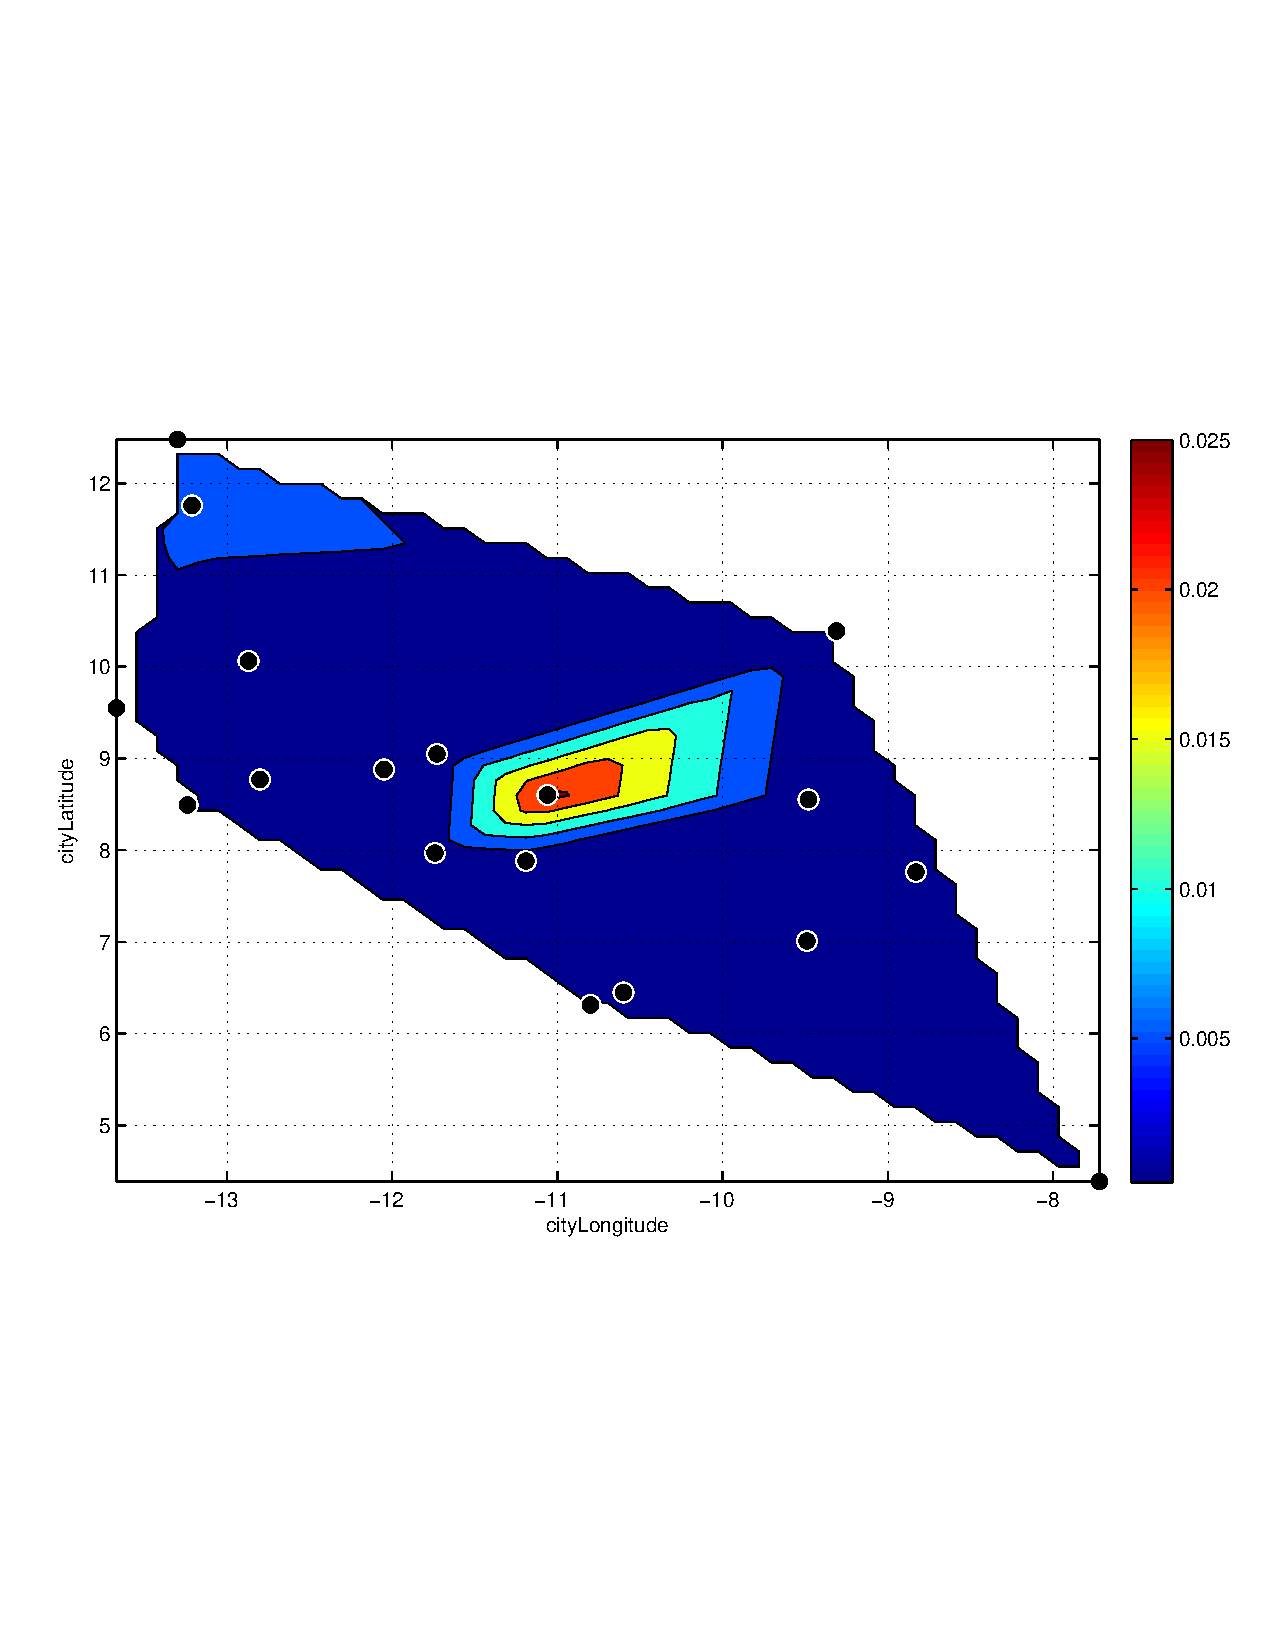
\includegraphics[width=0.6\textwidth]{vaccine_per_capita.pdf}
	\caption{The contour plot of vaccine per capita. The black spots represent locations of the 18 cities.}
	\label{vaccine_per_capita.pdf}
\end{figure}

\begin{table}[]
	\centering
	\begin{tabular}{|r|r|r|r|}
		\hline
		label of city & $drug_i$ & population of city & drug per capita ($\times 10^{-3}$) \\ \hline
		1             & 32       & 33190              & 0.9497                             \\ \hline
		2             & 111      & 167100             & 0.6643                             \\ \hline
		3             & 113      & 3222               & 34.9531                            \\ \hline
		4             & 93       & 1548000            & 0.060143                           \\ \hline
		5             & 112      & 772900             & 0.14476                            \\ \hline
		6             & 76       & 7461               & 10.1765                            \\ \hline
		7             & 59       & 45840              & 1.2819                             \\ \hline
		8             & 37       & 32660              & 1.1336                             \\ \hline
		9             & 14       & 114000             & 0.12545                            \\ \hline
		10            & 107      & 137700             & 0.78005                            \\ \hline
		11            & 31       & 117100             & 0.26779                            \\ \hline
		12            & 1        & 13990              & 0.077239                           \\ \hline
		13            & 6        & 43100              & 0.1433                             \\ \hline
		14            & 57       & 85020              & 0.67318                            \\ \hline
		15            & 108      & 1011000            & 0.10657                            \\ \hline
		16            & 22       & 1870               & 11.6608                            \\ \hline
		17            & 9        & 132700             & 0.067749                           \\ \hline
		18            & 12       & 21960              & 0.54899                            \\ \hline
	\end{tabular}
	\caption{A optimized plan for allocating drug with $drug_{tot} = 1800$ }
	\label{drug}
\end{table}

\section{Discussion}
\subsection{Strengths}
\begin{enumerate}
	\item \textbf{Our model is simple and easy to understand} \\
	      Our model is the simplest model we can conceive to reflect the impact of concerned independent variables (factors regarding medication) and to solve the problem lifted by the question.

	      Our single-city model is based on the most elegant model in the field of epidemiology - the SIR model, and we reconstruct the model (mainly add two clusters of people) in order to introduce concerned independent variable into our system.

	      Our multi-city model is based on our single-city model and introduce only one `people flow` to obtain the geographic characteristic of the spread of disease.

	\item \textbf{Our model is effective and in good agreement with the reality} \\
	      Simple as they are, they are effective in reflecting the complex relationships between numerous variables and parameters, and they not only reveal the intrinsic characteristics of the spread of disease itself but also successfully link factors of medication to the spread of disease.

	      Comparing with the data we have find from several resources, the results of our model not only correspond the general trend of the records but also resemble the reality in some critical features.

	\item \textbf{Good extensibility} \\
	      Flow of people is a critical factor determining the spread of disease. Although our multi-city model only set the volume of people flow as a function of mere geographic distribution and population of cities, the determinants of people flow can be adjusted when other possible factors are considered. Then, the adjusted model can be applied to study the impact of other possible factors relating to epidemiology.

\end{enumerate}



\subsection{Weaknesses}
\begin{enumerate}
	\item \textbf{Our model is just a rough model} \\
	      For simplicity, we have neglected many potential parameters, variables or processes, and have made numerous assumptions. Eg. we did not consider the relationship between separate individuals and we did not dig deeper into the properties of social network which is a quite essential part determining the spread of disease. Some important general or specific factors are also neglected by us, a interesting example of which is a folk custom prevalent in the studied region that relatives kiss the death, which plays a significant role in the spread of disease and is categorized into \emph{Super Spread Event}(SSE) academically.

	\item \textbf{Our model is only a continuous model} \\
	      Numbers of people, number of shares of drug/vaccine, etc. are important quantities in all the process of modeling and computation. For simplicity, we regard the numbers as directly real numbers instead of integers. It is justifiable when the numbers are large, since the decimal part of the number is negligible; when the system scales down, however, the statistics dose not work and the outcome deviates a lot from reality.
\end{enumerate}
\section{Conclusion}

In this paper, we have constructed our models based on the biological features of EVD, social features of human society and several reasonable assumptions. Our models consist of two parts: one is considering the the spread of disease within a single city and serves as the base of the other; the other takes the people flow among the cities into account, the application of which gives an optimized plan regarding how should we allocate the resources of medication such as vaccine.

Both of the models are applied to specific cases separately, and the results of computation which are carefully studied justified our model. Through our analysis of the model, we explored and explained the complex relationship among numerous variables and parameters.

The effectiveness of medical treatment ( including segregation, vaccination and pharmacotherapy ) is verified by our model and the strategy to allocate vaccine and drug is revealed by our investigation.
\section{Letter}
Dear readers,

In March 2014, the Ministry of Health of Guinea reported an outbreak of Ebola virus disease (EVD) in four southeastern districts: Guekedou, Macenta, Nzerekore and Kissidougou. A total of 86 suspected cases, including 59 deaths was reported as of March 24. Since then, the spread of EVD in West Africa has explosively grew. According to the latest statistics, EVD has caused 13855 cases and 9004 deaths. Faced with the havoc, the world have expressed their deep concern. In the last year, a mess of aid and donations converged on West Africa, medical orgnizations all over the world also dedicated to the researh of medication for EVD. With respect to people's determination of eradicating EVD, we now present our new progress on medication research.


The drug we developed aiming at EVD has been proved to have an amazing curative effect for the patients whose main organ hasn't been damaged. According to the data on clinical trial, 18 of 23 volunteers were cured, with an average recovery time of 8.4 days. It is gratifying that, with goverment's ratification, the drug has been put into mass production now. So patients will be able to receive effective medical treatment before long. The corresponding vaccine has also been developed, which is still in test stage. Vaccination against EVD can be expected soon.


However, as much as we might wish it, we can't provide the drug to all the patients without enough production capacity. To minimize the damage West Africa suffered, our only choice is to set cities' priority in drug delivery according to its population and location. Outbreak in populous cities is more destructive and uncontrollable, while cities near the epidemic focus stand a great chance of breaking out EVD. These cities will be firstly considered in our delivery system. Transportation hubs also have a high priority in our system as EVD may spread through transportation networks. Glacial as it sounds, this method has the highest efficiency in current situation. The latest arrangement details of medication delivery can be checked on our official website.

Though we are still in lack of effective medication, it is worth emphasizing that the confrontation against EVD needs not only medical researches, but also efforts of every single individual. A lot can be done to protect yourselves as well as others from infection. Some useful tips are given as follow

\begin{itemize}
	\item \textbf{Scale back on going out}
	      the transmission of EVD requires direct contact with the infected or their body fluids and blood. Reducing the contact with others is a proper way of avoiding infection.
	\item \textbf{Maintain personal hygiene}
	      This tip goes without saying. Personal hygiene is always of great significance even no epidemic disease is spreading. Maintain personal hygiene also means do not go to public places with appalling sanitary conditions.
	\item \textbf{Check data updates}
	      Keep focused on the data updates of EVD. This can help you get better acquainted with the situation and be prepared.
	\item \textbf{Be cautious}
	      If you feel uncomfortable, go to the medical institution nearby as soon as possible. You can suggest your friends to do the same. This act may prevent lives from fading away.
\end{itemize}

If you are unfortunately infected with EVD, don't panic. EVD is not absolute lethal. You can still stand a good chance of recovery as long as doctor's advices are followed.

The status of fighting against EVD remains severe now, and we will continue our efforts in medication development and medical assistance. To our belief, EVD will be thoroughly eradicated in the near future.
\begin{thebibliography}{99}
	%\addcontentsline{toc}{section}{References}

	\bibitem{SIR}Kermack W O, McKendrick A G. A Contribution to the Mathematical Theory of Epidemics[J]. Proceedings of the Royal Society of London. Series A, 1927, 115(772):700-721.
	\bibitem{SIS}W. O. Kermack , A. G. McKendrick   Contributions to the mathematical theory of epidemics. Proc Roy Soc,1932:(A138):55-83
	\bibitem{yuzhi}Lipsitch I , Cohen T , Cooper B , Transmissions Dynamics and Control of Severe Acute Respiratory Synddrome[J]. Science 10, 1126;1086616(2003 May 23)
	\bibitem{SEIR}Dye C , Gay N . Modeling the SARS epedemic. Science, 2003;300:1884-1885
	\bibitem{GIS}AsehwandenC.Spatial simulation model for infectious viral diseases with focus on SARS and the common flu. Proceedings of the 37th Hawaii International Conference on System. Science,2004
	\bibitem{CDC}Website of Centers for Disease Control and Prevention: \emph{http://cdc.gov.com}
\end{thebibliography}

%====================附录导入程序代码==========================================
\begin{appendices}
    %\renewcommand{\thesection}{\Alph{chapter}.}

\section{First appendix}

some text...


Here are simulation programmes we used in our model as follow.\\


\textbf{\textcolor[rgb]{0.98,0.00,0.00}{Input matlab source:}}
\lstinputlisting[language=Matlab]{./code/matlab1.m}


      \section{Second appendix}

    some more text \textcolor[rgb]{0.98,0.00,0.00}{\textbf{Input C++ source:}}
\lstinputlisting[language=C++]{./code/sudoku.cpp}

\end{appendices}

\end{document}